\chapter{Signal measurements}

By the time the \gls{rf} signal has reached the piezoelectric of the
\gls{aod} it has been synthesized from a reference signal, amplified to match
the power requirements of the \gls{aod} and matched to the impedance of the
\gls{aod}. Each of these stages ammends the shape of the \gls{rf} signal and
as we will see introduce new frequency responses of the amplitude. The so
inevitable amplitude modulation affects the deflected intensity of the laser
beam and will lead to the intensity characteristics discussed in the next
chapter.

\section{Digital signal synthesis}

As has been described in the experimental setup section, \gls{dds} are used
for signal synthesis. In the present section we want to examine the
frequency behaviour of the \gls{dds}. In particular we are interested how the
amplitude responds to different frequencies and how the digital design of the
\gls{dds} affects the \gls{rf} signal shape.

\subsection{Setup}
\label{subsec:signal_synthesis_setup}

For the following experiments we configured the \gls{dds} to do a linear
frequency sweep from \SI{80}{\mega\hertz} to \SI{120}{\mega\hertz} at a sweep
duration of \SI{26.84}{\micro\second}. The frequency range has been choosen
because it overlaps with the operation range required to drive the \gls{aod}.
The sweep duration is a good compromise between being able to resolve the
complete sweep with limited oscilloscope resolution on the one hand and
limited frequency resolution of the synthesizer.

The time resolution of most oscilloscopes depends on the selected time scale,
however choosing a finer time scale entails shortening the time length, thus
we have a trade-off between being able to perform signal analysis that demands
fine resolution of the sinusoidal voltage and the number of measurements we
need to perform to capture a complete passthrough of the synthesized signal
cycle. We found that a selected time division of \SI{10}{\micro\second} is
sufficient for signal analysis, i.e. \gls{fft}, but at the same time limits
the number of measurements to the magnitude of hundreds.

To overcome the obstacle that we can only capture one time window of a
\gls{rf} signal passthrough we inserted a frequency generator between the
external trigger source and the oscilloscope. The frequency generator is
configured to emit a square wave pattern on the rising edge of the external
trigger of width $d$. The oscilloscope was configured to be triggered on the
falling edge of the external trigger signal supplied by the frequency
generator. By adjusting the square wave width $d$ we effectively added a
delay to the trigger signal. In order to capture now the complete signal over
duration $T$ we incremented the delay $d$ in steps of $T/300$.

\subsection{Results}
\label{subsec:signal_synthesis_results}

The former setup produced a single dataset we evaluated from two different
angles. First we explored how the digital design of the \gls{dds} propagates
into the signal. Second we explored the frequency dependence of the amplitude.

\subsubsection{Spectrogram}

A spectrogram visualizes how the frequency spectrum varies in time. One way
to obtain a spectrogram is to partition the data into overlapping time chunks
while performing \gls{fft} which allows us to combine time and frequency
domain specific characteristics. In our case we choose the relative spectral
power to be encoded through color.

\begin{figure}[h]
  \centering
  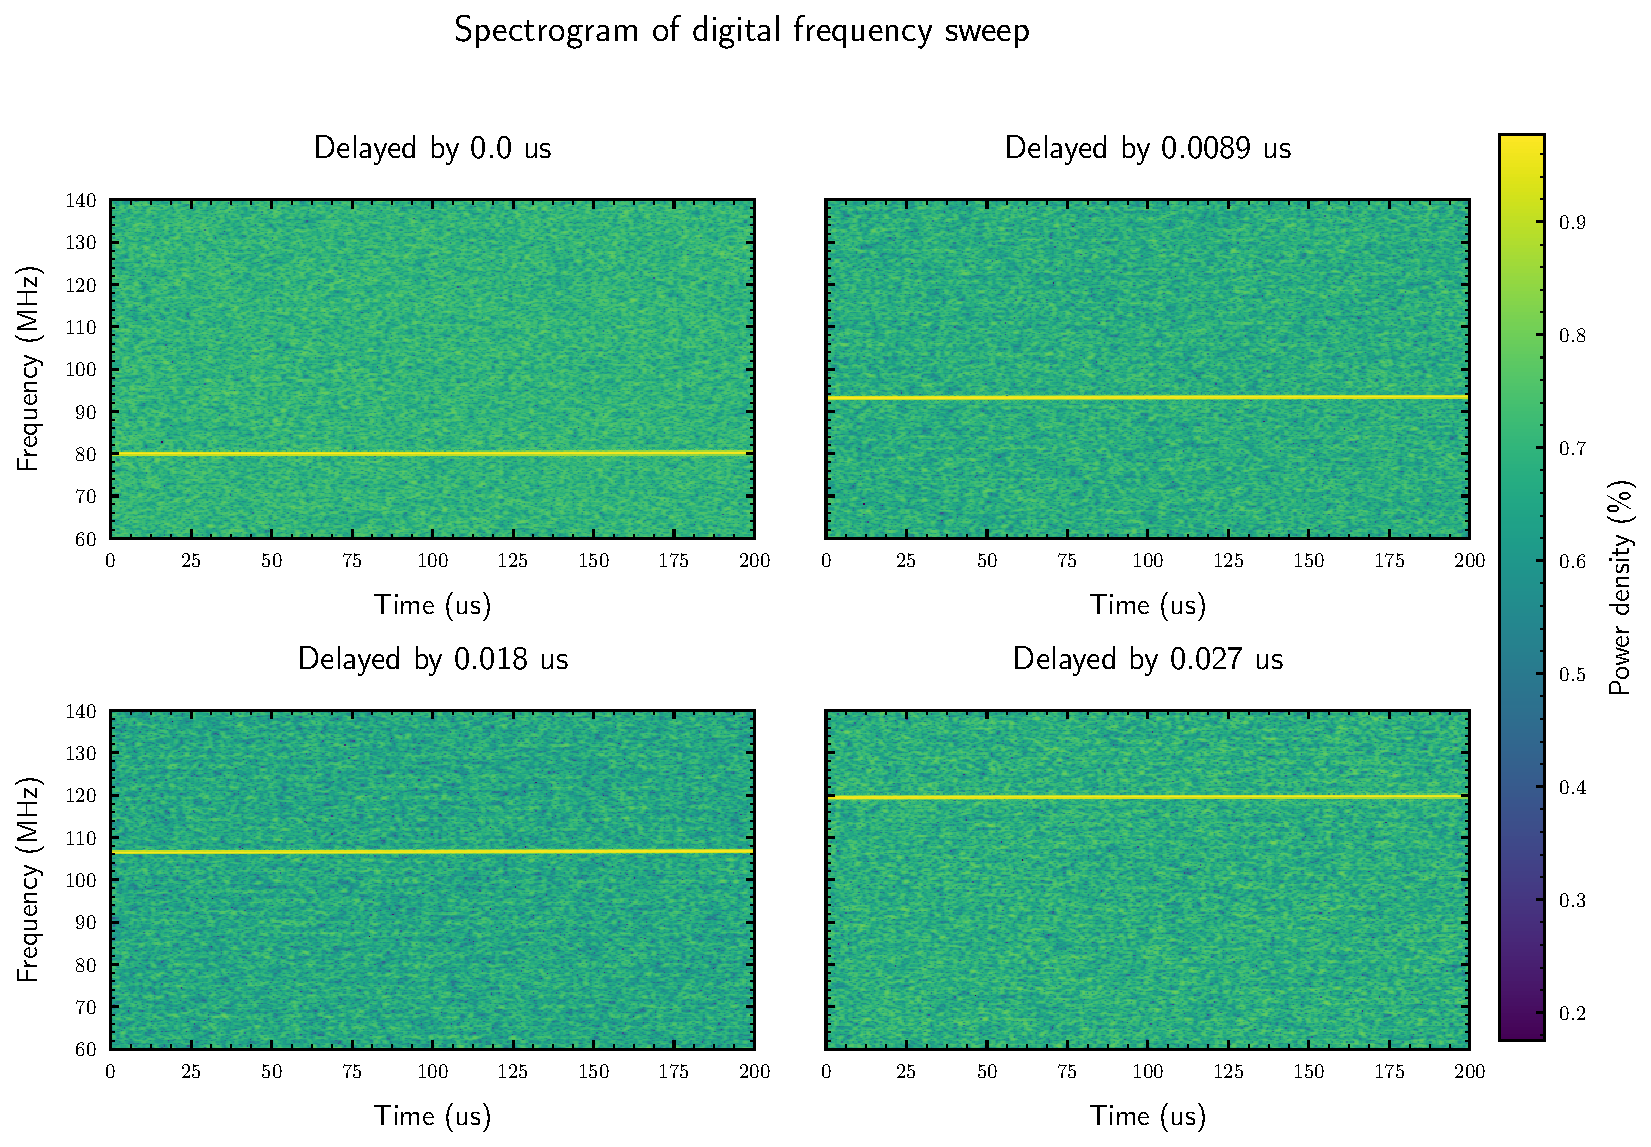
\includegraphics[width=\textwidth]{\figuredir{signal/synthesis/spectrogram.pdf}}
  \captionsetup{width=.8\textwidth}
  \caption{Spectrogram of delayed time windows of the \gls{dds} output signal
    configured to perform a frequency sweep from \SI{80}{\mega\hertz} to
    \SI{120}{\mega\hertz}. For an ideal linear sweep we would expect a linear
    timeline of the frequency, instead we observe a discrete set of
    frequencies which reflects the digital nature of the \gls{dds}.}
  \label{fig:signal_synthesis_spectrogram}
\end{figure}

\Cref{fig:signal_synthesis_spectrogram} depicts four spectrogram, each taken
at a different time window of the frequency sweep passthrough. The first
spectrogram captures the start of the frequency sweep. We can see how for the
first \SI{200}{\micro\second} the \gls{dds} outputs only the start frequency
of \SI{80}{\mega\hertz} which then is increased by increments to reach the
final frequency of \SI{120}{\mega\hertz} as can be seen in the lower right
spectrogram at the end of the frequency sweep.

For an ideal frequency sweep we would expect a linear timeline of the
frequency, instead we see that \gls{dds} outputs a discrete set of
frequencies.

\subsubsection{Amplitude frequency response}

Although the previous section satisfied our curiousity it did not disclose
anything we did not expect. Anyhow, in this part we examine the amplitude
frequency response which by all means has great significance on the observed
intensity patterns we discuss later.

\begin{figure}[h]
  \centering
  \includegraphics[width=\textwidth]{\figuredir{signal/synthesis/frequency-max-amplitude.pdf}}
  \captionsetup{width=.8\textwidth}
  \caption{Maximum amplitude of the two \gls{dds} at different frequencies
  during linear sweep operation. In the two lower curves the \gls{dds} were
configured with enabled inverse sinc filter that is supposed to compensate
frequency dependence in the amplitude.}
  \label{fig:signal_synthesis_frequency_max_amplitude}
\end{figure}

To find the frequency dependency of the amplitude we carried out \gls{fft} on
the voltage of the respective time window and extracted the dominant
frequency located at the maximum of the power spectrum and thereby reduced
each measurement to a frequency and corresponding maximum amplitude.

The result is visualized for the two different signal sources with different
filter mode in \Cref{fig:signal_synthesis_frequency_max_amplitude}. We observe
that there is no significant difference between distinct \gls{dds}. The
inverse sinc filter proclaimed to reduce frequency dependence of the amplitude
only reduced the output amplitude without changing the overall frequency
response characteristics.

\subsection{Summary}

At the signal source stage the \gls{dds} already induce significant frequency
dependency of the output amplitude. The built-in inverse sinc of the \gls{dds}
does not reduce this dependency, therefore we disable the inverse sinc
filter for all other measurements. Eventually we could confirm the
discreteness of the frequency domain produced by the \gls{dds}.

\section{Signal amplification}

The \gls{rf} signal supplied by the synthesizer is too weak to power the
\gls{aod}, therefore we supply the synthesized signal to an amplifier and
feed the amplified signal to the \gls{aod}. The amplification acts as the
second stage in our \gls{rf} signal processing and we expect it to amend
the frequency behaviour of the amplitude.

\subsection{Setup}

The measurement algorithm described in \cref{subsec:signal_synthesis_setup} is
still valid for the now amplified signal. Even though we found in the former
section that the synthesized signal does not differ in between different
\gls{dds} we supplied the horizontal \gls{dds} to the respective amplifer.

The amplified signal should be of approximate power \SI{33}{\decibel\meter}.
At the usual \SI{50}{\ohm} in between coaxial cables this corresponds to an
approximate voltage of \SI{10}{\volt}. Even though the employed oscilloscope
is rated for more then \SI{10}{\volt} when being used in \SI{1}{\mega\ohm}
mode we inserted a chain of attentuators (from coaxial cable to
oscilloscope: \SI{1}{\decibel}, \SI{3}{\decibel}, \SI{6}{\decibel},
\SI{10}{\decibel} and \SI{10}{\decibel} to distribute heat dissipation) in
between the coaxial cable and the oscilloscope input to attain a total
damping of \SI{30}{\decibel}.

\subsection{Results}

The analysis is analogue to the frequency response part in
\cref{subsec:signal_synthesis_results} in that we perform \gls{fft} on each
measurement window to extract the dominant frequency with the maximum
amplitude in the time domain. The maximum amplitude is very close to the
effective amplitude of a sinusoidal signal, yet it is much easier to extract
from the time series data.

In a second step we normalized the so obtained amplitude frequency response
of the amplified signal with the previously evaluated source signal amplitude
frequency response. The specific normalization used was a min-max type where
we subtracted the minimum amplitude from each signal and divided the
difference by the new value range.

The spectrogram of the amplified signal should be equal to
\Cref{fig:signal_synthesis_spectrogram}, hence not give us any new insights.

\subsubsection{Amplitude frequency response}

\Cref{fig:signal_amplification_frequency_max_amplitude} presents us the
damped output signal subject to the signal frequency after amplification for
the two distinct amplifiers. We require two distinct amplifiers because our
setup comprises two independently controlled \gls{aod}.

\begin{figure}[ht]
  \centering
  \includegraphics[width=\textwidth]{\figuredir{signal/amplification/frequency-max-amplitude.pdf}}
  \captionsetup{width=.8\textwidth}
  \caption{Maximum amplitude at dominant frequency per delayed window for two
  different amplifiers. We can see the discreteness of the frequency domain
from the digital signal synthesis as well as three resonances. Further the
amplifier differ by a constant offset.}
  \label{fig:signal_amplification_frequency_max_amplitude}
\end{figure}

At first we note that the amplified signal differs by a constant offset. We
assume this offset to be caused by different component quality as the
frequency response shape itself is similar. On a
second glance we again find evidence for discrete frequencies from
\Cref{fig:signal_amplification_frequency_max_amplitude} when we emphasize the
subtile horizontal pattern of the markers.

\subsubsection{Comparison with source signal}

\Cref{fig:signal_amplification_comparison} shows the min-max-normalized
amplified signals with the min-max-normalized input signal from the horizontal
\gls{dds}. After normalization the fixed offset difference, we observed
previously in between the distinct amplifiers, vanishes and the same
frequency response shape is obvious.

\begin{figure}[ht]
  \centering
  \includegraphics[width=\textwidth]{\figuredir{signal/amplification/comparison.pdf}}
  \captionsetup{width=.8\textwidth}
  \caption{Relative amplitude at dominant frequency per delayed window for
  two different amplifiers and their digital signal source. In comparison to
the signal source the amplifiers introduce a further resonance at the
center frequency.}
  \label{fig:signal_amplification_comparison}
\end{figure}

Comparison of the signal after (black, green) and before amplification (red)
yields that the input signal from \gls{dds} seems more dense than after the
amplification, yet we miss a solid explaination for this behaviour as the
amplification process uses analogue components. It could be that the voltage
resolution of the oscilloscope was misconfigured to a to coarse scaling.
Furthermore we observe that the amplifier remedies the amplitude drop
at around \SI{102}{\mega\hertz} of the source signal. However the amplifier
possess resonacnes around \SI{98}{\mega\hertz} and \SI{110}{\mega\hertz}
where the amplitudes drop.

\subsection{Summary}

To sum up we found that distinct amplifier differ by a fixed voltage offset.
Furthermore the amplifiers introduce new resonances into the amplitude
frequency response and posseses a more discrete signal spectrum then the
input signal.

\section{Signal reflection}

In the previous sections we explored the signal transfer at the synthesis
and amplification stage. The last stage that is accessable to us without
destruction of the \gls{aod} concernse the power reflection at the \gls{aod}
itself. From the reflection we can deduce the power transmission, hence for
a large reflection we would expect a small transmission and in that sense
less beam intensity in the first deflection order.

\subsection{Setup}

The power reflection measurements were conducted with a network analyzer. In
a first embodiment of the experiment we directly supplied the \gls{aod}
through a coaxial cable of the network analyzer with power and measured the
reflection. In a second embodiment we used a direct-coupler to supply the
respective amplifier with a signal and measure the reflection through the
direct-coupler to avoid harm to the network analyzer because the network
analyzer is not able to provide \SI{2}{\watt} of output power as required
by the \gls{aod}.

\subsection{Results}

At first we discuss the reflection spectrum of the direct connection of
the network analyzer and the distinct \gls{aod} elements. Thereafter we
analyze the reflection spectrum of the direct-coupler and then continue with
the reflection spectrum with an amplified signal. Finally we compare the
direct and amplified spectra.

\subsubsection{Direct connection}

\Cref{fig:signal_reflection_direct} visualized the power reflection spectrum
of both \gls{aod} elements when direct coupled to the network analyzer at
the maximum output power of \SI{10}{\decibel\meter}.

\begin{figure}[ht]
  \centering
  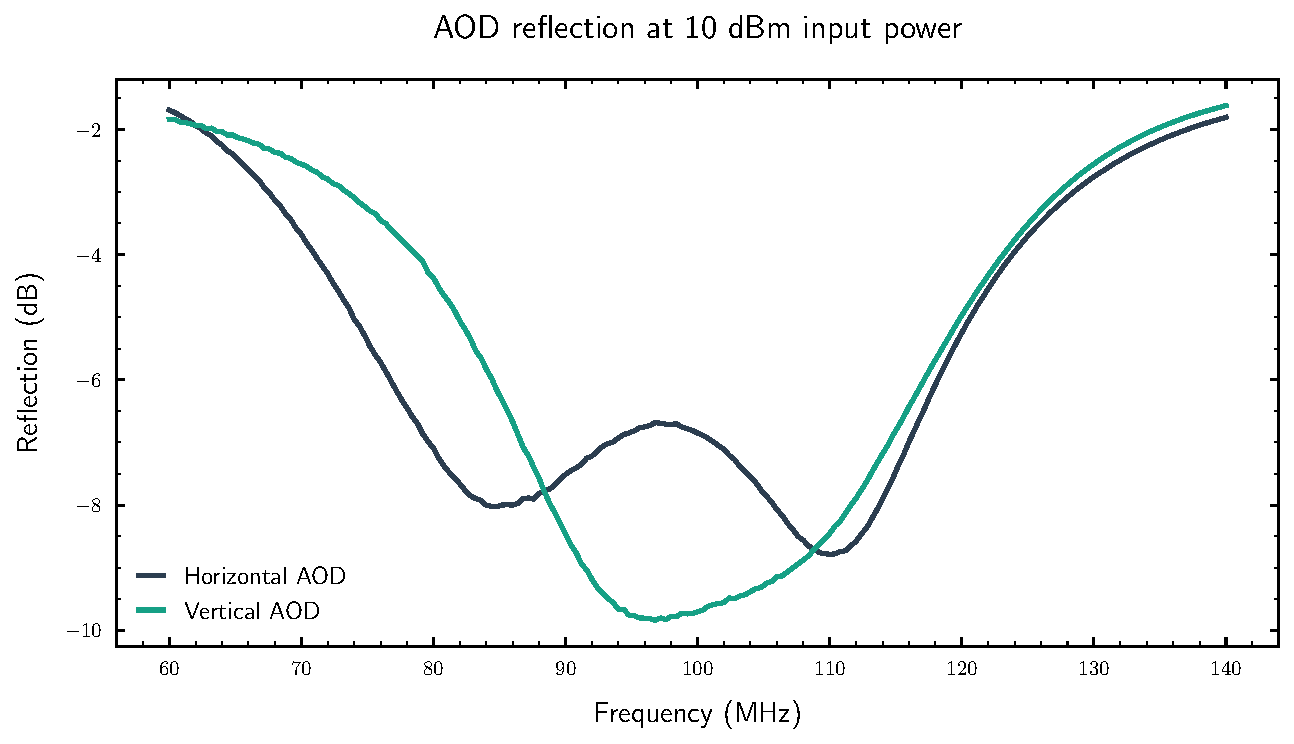
\includegraphics[width=\textwidth]{\figuredir{signal/reflection/direct.pdf}}
  \captionsetup{width=.8\textwidth}
  \caption{We see the signal reflection of the two different \gls{aod} when
  connected directly to the network analyzer. We can see that both crystal
differ in their respective spectrum.}
  \label{fig:signal_reflection_direct}
\end{figure}

Most interesting finding in \Cref{fig:signal_reflection_direct} is that the
power reflection shows very different behaviour in between the distinct
\gls{aod} elements. The \gls{aod} anticipated for the vertical deflection
is most transmissive at \SI{97}{\mega\hertz} with transmission falling of
on both sides while the \gls{aod} anticipated for the horizontal deflection
has two local transmission maxima and a rather bad transmision near the center
frequency.

\subsubsection{Direct-coupler}

The direct-coupler is an apparatus comprising a coaxial input and output
port as well as a coaxial input reflection and output reflection port. It is
disignated to measure the reflection of a (possible) high power signal
without jeopardizing measurement equipement.

\begin{figure}[ht]
  \centering
  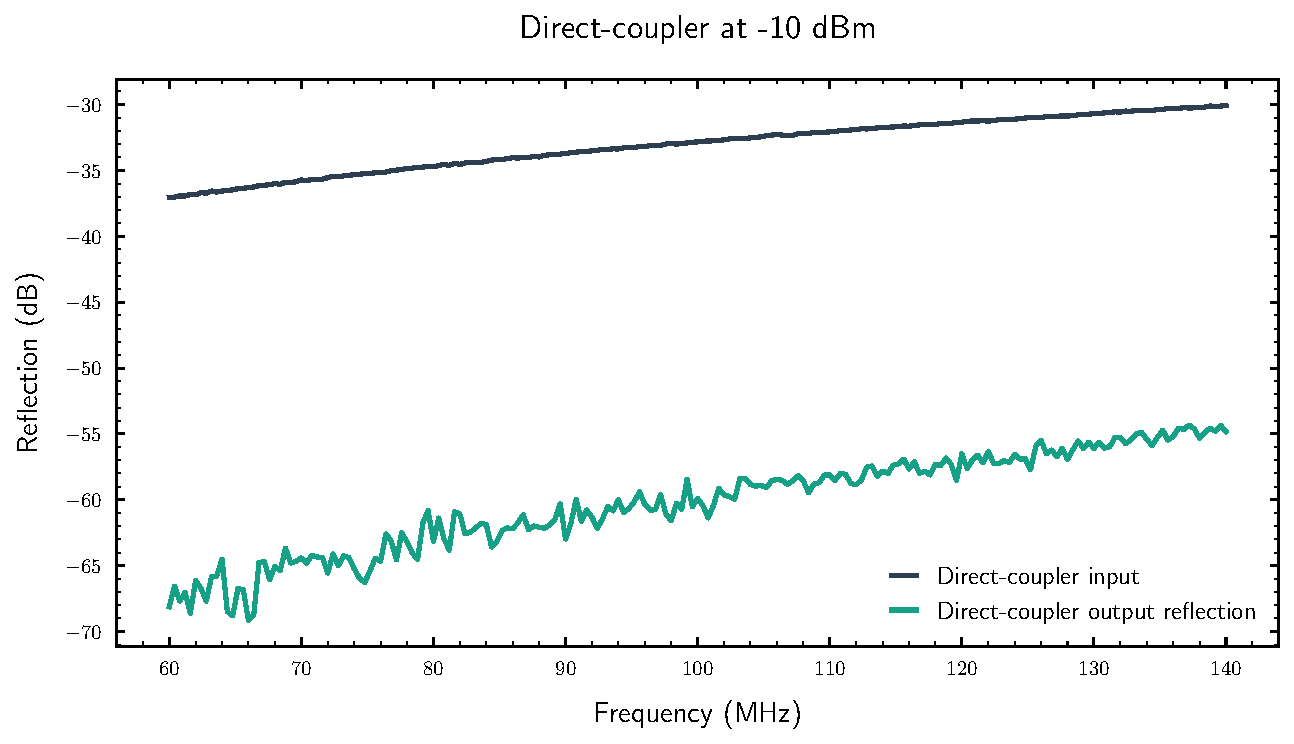
\includegraphics[width=\textwidth]{\figuredir{signal/reflection/coupler.pdf}}
  \captionsetup{width=.8\textwidth}
  \caption{Input power reflection when supplying the direct-coupler with
    \SI{-10}{\decibel\meter} input signal and reflection at the output of
    the direct-coupler while other ports are closed with \SI{50}{\ohm}}.
  \label{fig:signal_reflection_coupler}
\end{figure}

In \cref{fig:signal_reflection_coupler} we see the reflection spectrum for
the case that we provide the network analyzer output signal to the input of
the direct-coupler and connect the reflection output of the direct-coupler
with the second network analyzer port while the remaining ports are under
\SI{50}{\ohm} closure.

We note that the reflection measured at through the direct-coupler is lowered
by many orders of magnitude compared to the input signal but essentially of
the same shape. The noise in the reflection is very high because of the low
power supplied into the direct-coupler.

\subsubsection{Amplification coupled}

We now use the direct-coupler to measure the output reflection at the
\gls{aod} elements after the signal was amplified.

\begin{figure}[ht]
  \centering
  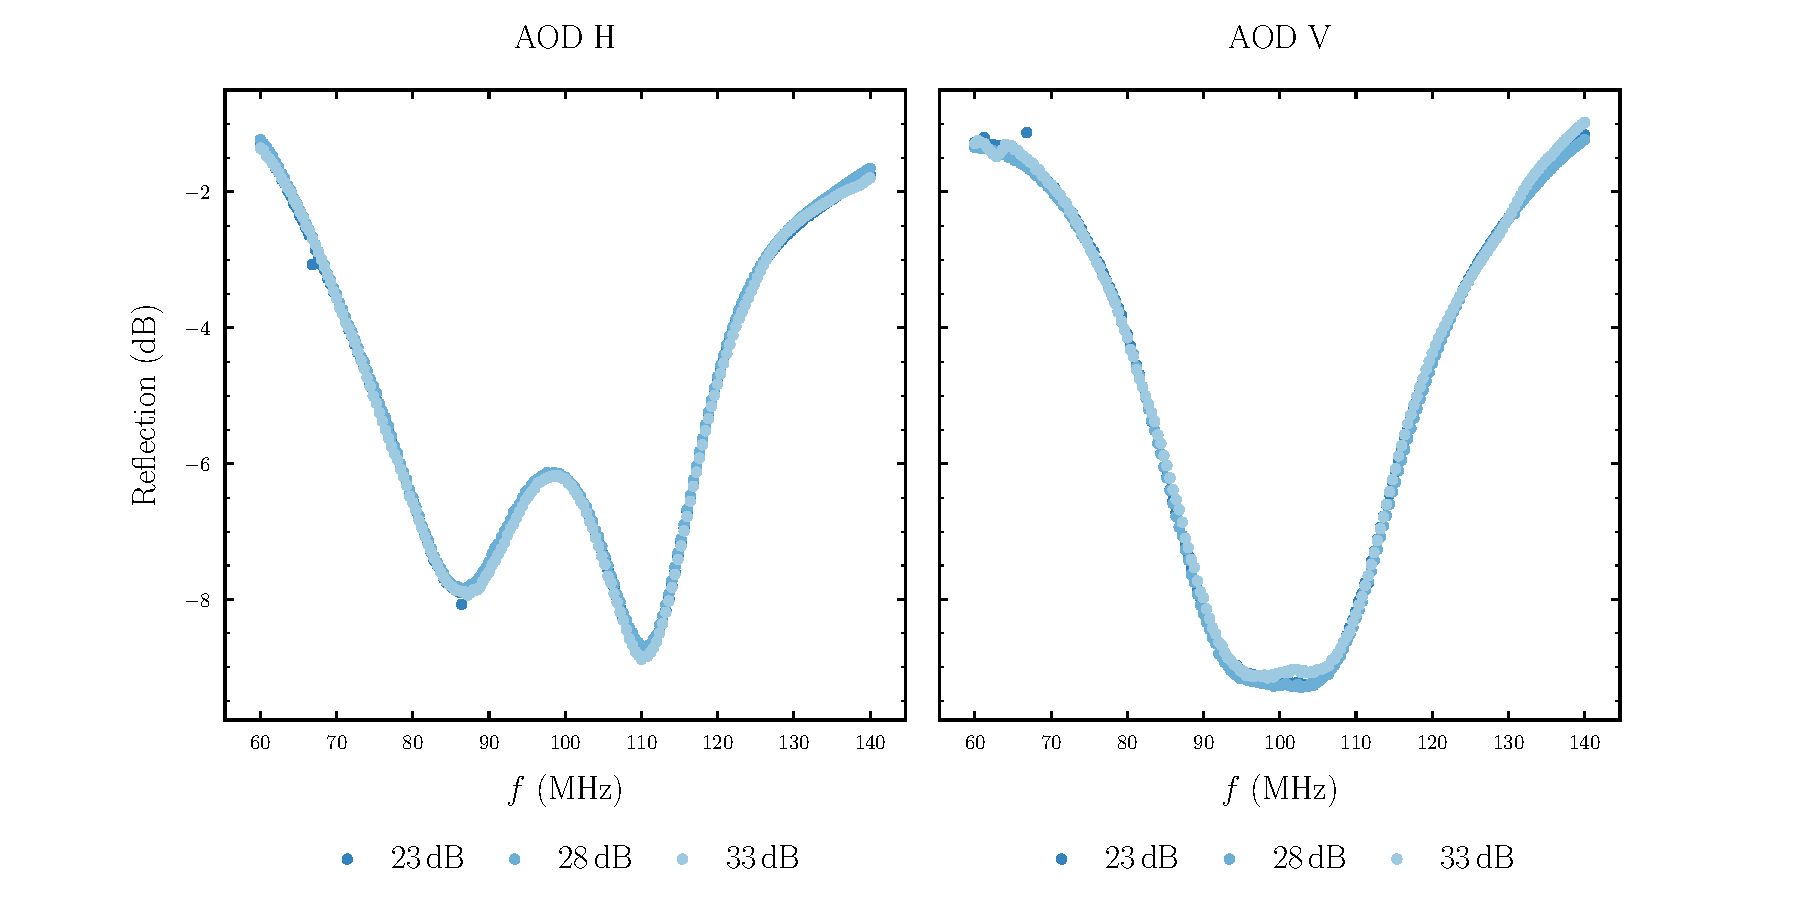
\includegraphics[width=\textwidth]{\figuredir{signal/reflection/coupled.pdf}}
  \captionsetup{width=.8\textwidth}
  \caption{Reflection at the direct-coupler output after amplification of the
  network analyzer input signal for different effective powers. We see that
the applied power does not effect the spectrum.}
  \label{fig:signal_reflection_coupled}
\end{figure}

In \Cref{fig:signal_reflection_coupled} we see the effective reflection
spectrum for the distinct \gls{aod} elements. The effective reflection
spectrum is obtained when subtracting the input reflection from the output
reflection.

\subsubsection{Comparison}

In the previous part we saw that the reflection spectrum does not show any
power dependence, thus we should be able to compare the spectrum we obtained
directly with the amplified result.

\begin{figure}[ht]
  \centering
  \includegraphics[width=\textwidth]{\figuredir{signal/reflection/comparison.pdf}}
  \captionsetup{width=.8\textwidth}
  \caption{Comparison of reflection from amplified input signal and direct
  signal provided from the network analyzer. The different reflection spectrum
can be associated to the amplifier.}
  \label{fig:signal_reflection_comparison}
\end{figure}

In \Cref{fig:signal_reflection_comparison} we can see how there is additional
reflection from the amplifier, nevertheless the global spectrum
characteristics stay in place.

\subsection{Summary}

Distinct \gls{aod} elements show different power transmission characteristics
and the amplifier only causes marginal shifts. Examination of the \gls{aod}
elements in details discloses different impedance matching circuits.

Impedance matching is used to reduce power reflection by providing a constant
input resistance of \SI{50}{\ohm} accross an ideally wide frequency range.
Still the impedance differs between the \gls{aod}s. We assume that the
crystal properties i.e. cut, purity are responsible for that.

By the previous reflections measurements we keep in mind that these were
conducted with an input signal with fairly homogenous amplitude. From the
previous sections we know that this in fact is not the case for the \gls{rf}
signal later used.
